\section{Sviluppo dell'applicativo} \label{software}

L'applicativo è stato realizzato per mezzo di scripting python \cite{pydoc}, su sistema operativo GNU/Linux, in particolare sotto la versione Ubuntu Linux 8.04. Si è trattato con buoni risultati i casi più diffusi di bibliografia che utilizzano una struttura standard benformata per elencare le varie voci. Si è riusciti a trattare con risultati sufficienti anche i casi in cui la bibliografia non segue una regola predefinita.

Estratta la bibliografia sono state implementate delle funzioni che effettuano richieste SOAP al WebService di Google \cite{GWS} per mezzo di proxy in python \cite{ibm-py-ws} utili sia a correggere il titolo tramite Google Suggest sia a recuperare la Url della risorsa Web con maggiore ranking, correlata alla voce bibliografica. 

Infine sono state sviluppate delle funzioni che costruiscono un file HTML contenente tutte le voci della bibliografia con il link remoto e l'eventuale BibTex estratto dalla pagina HTML della risorsa remote come ad esempio CiteSeer, Portal ACM etc. L'ultima caratteristica aggiunta all'applicativo è quella di poter scaricare alcuni pdf citati e organizzarli in una cartella. Il download dei pdf citati è però solo stati possibile in quei pochi portali liberi di accesso e non a pagamento.

In figura sottostante sono riportati i passi princiapli dello script che vengono eseguiti:
\begin{enumerate}
	\item Estrazione del testo
	\item Implementazione dell'euristiche basate su espressioni regolari per localizzare la bibliografia ed estrarre le voci
	\item Estrazione dei titoli
	\item Scrittura del file html con l'eventuale ricerca via webservice. 
\end{enumerate}


\begin{lstlisting}[frame=r,caption=Il File principale - pdftoref.py ,breaklines=true,basicstyle=\small]{}

# Si estrae il testo dal Pdf in formato XML
document = Pdf2Txt.getTextFromPdf(content)

# Si estrae la bibliografia dal file XML come testo semplice
plainText = Extractor.getPlainText(document)

if plainText:
	# Si cerca di estrarre le varie voci della bibliografia 
	entries = Extractor.entriesExtractor(plainText)
	if entries:
		# Si scrive ciascuna entry in un file HTML col relativo collegamento
		HtmlWriter.write(entries,titles,content,urlFlag,bibtexFlag)

\end{lstlisting}

\subsection{Estrazione Testo Pdf}
Il primo problema che si presenta nell'estrazione dei dati dal file Pdf è stato l'estrazione del testo. Pdf è un formato di stampa e talvolta tratta il testo alla stregua di immagini. In alcuni casi descrive le lettere di una stessa parola in maniera diversa dalle altre per ottenere un buon risultato di stampa, ma restitudendo un pessimo risultato per l'analisi del testo. Non è facile perciò ottenere un \textit{clear plain text} da un file Pdf. Tuttavia sono presenti un numero di tools e librerie che svolgono questa funzione in modo più o meno appropriato, a seconda delle esigenze dell'utente. Ci sono dei tools che dato un file PDF restituiscono un file XML che contiene oltre al testo la descrizione della formattazione del documento. 
In particolare si è analizzato e testato tre strumenti diversi:
\begin{itemize}
 \item \textit{pdftohtml} è un applicativo, distribuito come \textit{free software}, a linea di comando in dotazione con praticamente qualsiasi distribuzione GNU/Linux. E' utile per la conversione di un file pdf in html o xml e abbstanza veloce in quanto scritto in C++.
 \item \textit{PyPdf} è una libreria python utile per la manipolazione di documenti pdf, estrae testo semplice. Permette di fare \textit{merge} di pdf, ruotarli e tagliarli.
 \item \textit{PDFMiner} è una suite di programmi sviluppata completamente in python, scritta da Yusuke Shinyama, che implementa funzionalità di estrazione testo e formattazione da files pdf. In particolare fornisce la possibilità di ottenere un file xml equivalente al pdf.
\end{itemize}

Sottolineando che si è ricercato tutti strumenti al limite con una licenza opensource\footnote{ricordarsi di citare i siti di questi progetti}, la scelta è infine caduta sulla suite PDFMiner perchè è scritta completamente in python e perciò meglio integrabile col nostro progetto, è funzionale per i nostri obiettivi ed è di semplice applicazione pratica.
In particolare PDFMiner offre un interfaccia python direttamente integrabile con altro software python, per questo ci ha permesso di raggiungere l'obiettivo con un numero esiguo di modifiche al codice: solo la creazione di un file di binding tra il tool e l'applicativo pdftoref. La funzione di binding prende il nome \texttt{getTextFromPdf(PdfFile)} e ritorna un documento XML benformato di questo tipo:

\begin{lstlisting}[language=XML,frame=r,caption=Esempio di XML relativo a documento PDF ,breaklines=true,basicstyle=\small]{Esempio di XML relativo a documento PDF}
...
<document>
 <page id="0" bbox="92.381,119.270,429.987,660.000" rotate="0">
  <text font="DMFDHG+CMBX12" direction="1" bbox="134.765, 361.365,  62.920, 11.955" size="11.955">References</text>
  <text font="DMFDIK+CMR9"   direction="1" bbox="139.372, 340.543, 341.146,  8.966" size="8.966">1. J.-F. Arias, C.P. Lai, S. Surya, R. Kasturi, and A.K. Chhabra. Interpretation of</text>
  <text font="DMFDIK+CMR9"   direction="1" bbox="140.727, 339.321, 148.241,  8.966" size="8.966">telephone system manhole drawings.</text>
  <text font="DMHOKA+CMTI9"  direction="1" bbox="157.848, 339.339, 111.177,  8.966" size="8.966">Pattern Recognition Letters</text>
  <text font="DMFDIK+CMR9"   direction="1" bbox="170.248, 339.321,  64.383,  8.966" size="8.966">, 16(1):355&#8211;359,</text>
  <text font="DMFDIK+CMR9"   direction="1" bbox="140.727, 338.099,  20.990,  8.966" size="8.966">1995.</text>
 </page>
</document>
...
\end{lstlisting}



\subsection{Ricerca References}

Ottenuto il file XML è necessario operare una ricerca nel testo per selezionare il testo relativo alla bibliografia.
Per fare ciò ci siamo basati sui seguenti criteri:
\begin{itemize}
 \item Negli articoli in inglese la bibliografia inizia sempre con la parola \textit{``Reference''} o \textit{``References''}.
 \item Negli articoli in inglese la bibliografia si trova sempre nella parte finale.
\end{itemize}

Perciò abbiamo operato una ricerca dal fondo del documento (\textit{bottom-up}) come in Figura \ref{fig:bottomup} al fine di trovare la prima occorrenza della parola \textit{``Reference''} alla quale abbiamo supposto seguire soltanto il testo relativo alla bibliografia. 
Un problema pratico che si è affrontato qui è dovuto all'estrazione del testo dal pdf. La parola ''References'' infatti'' non è sempre estratta in modo coerente a causa delle problematiche nell'analisi del testo del formato di stampa PDF citate precedentemente. Infatti potrebbe presentarsi come ''Re fe rence'' o ``R e ference'', insomma con degli spazi all'interno. Per ovviare a ciò ci siamo avvalsi delle\textbf{ espressioni regolari} in python, uno strumento molto efficacie per la manipolazione e l'analisi del testo.

\begin{figure}[htb]
\begin{center}
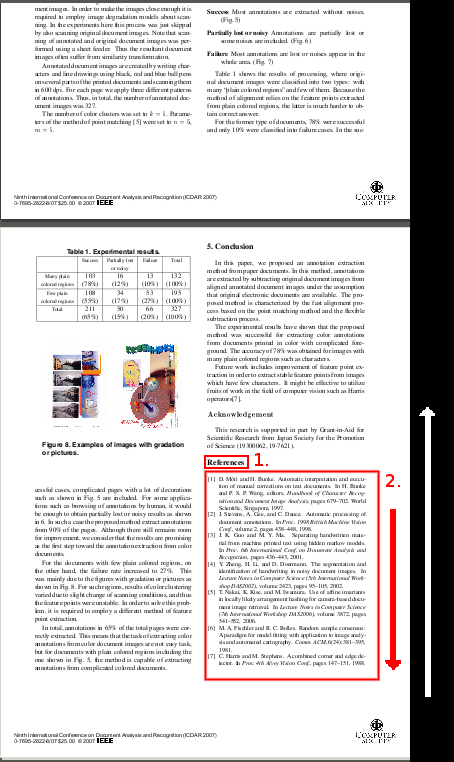
\includegraphics[scale=0.45]{bottomup.png}
\end{center}
\caption[Rappresentazione grafica di ricerca bottom-up]{Rappresentazione grafica di ricerca bottom-up: la ricerca è fatta prima sull'espressione regolare References (.1) dal bbasso verso l'alto del documento. Una volta trovata si ritorna indietro supponendo che tutto il testo da References in giù sia la bibliografia (2.) }
\label{fig:bottomup}
\end{figure}

\begin{subsubsection}{Espressioni Regolari}
 Le espressioni regolari (in inglese \textit{regular expression} \cite{regexp}, che può trovarsi abbreviata in regexp, regex o RE) sono grammatiche di tipo 3, cioè della tipologia più semplice. Sono uno strumento molto potente e abbastanza flessibile con cui si possono rappresentare un insiemi di stringhe. Gli insiemi caratterizzabili con espressioni regolari sono anche detti linguaggi regolari (e coincidono con quelli generabili dalle grammatiche regolari e riconoscibili dagli automi a stati finiti). Le espressioni regolari sono composte da costanti e operatori che denotano insiemi di stringhe, e da operazioni tra questi insiemi. Le espressioni regolari sono utilizzate principalmente da editor di testo per la ricerca e la sostituzione di porzioni del testo. Grande importanza rivestono inoltre nell'informatica teorica, nella quale, ad esempio, sono utilizzate per rappresentare tutti i possibili cammini su un grafo.

Le espressioni regolari operano sulle stringhe, e le stringhe più semplici sono costituite da singoli caratteri. La maggior parte dei caratteri corrisponde semplicemente a se stessa, quindi a corrisponderà alla stringa "a" (circa la discriminazione tra maiuscolo e minuscolo si veda la sezione opzioni più avanti), stessa cosa per una stringa costituita da caratteri ordinari, come a esempio spam.

Alcuni caratteri assumono invece significati particolari e vengono chiamati \textit{metacaratteri}. Laddove si voglia vengano interpretati come caratteri ordinari dovranno essere protetti. Eccone una lista completa:

\begin{verbatim}
[ \ { | ( )  ^ $ ? + * .
\end{verbatim}

Il metacarattere \textit{*} specifica che la RE che lo precede (può essere un singolo carattere, ma a esempio anche un intervallo [a-z]) può ripetersi zero o più volte, quindi a esempio pip*o trova corrispondenza in ``pio'' (zero ``p''), ``pipo'', ``pippo'', ``pipppo'' e così via.\\

Simile è il comportamento di \textit{+}, che specifica che la RE che lo precede può ripetersi una o più volte (attenzione a tale differenza!). Quindi pip+o troverà corrispondenza in ``pipo", ``pippo'', ``pipppo'' e così via, ma non in ``pio'' (al minimo una ``p'').\\

Più ristretto è il comportamento di \textit{?}, che specifica che la RE che lo precede può ripetersi zero o una volte. Quindi la nostra pip?o troverà corrispondenza solo in ``pio'' o ``pipo''.\\

\textbf{Esempio di utilizzo nella nostra applicazione}
\begin{lstlisting}[frame=r,caption=Esempio di utilizzo di espressione regolare per la ricerca ,breaklines=true,basicstyle=\small]{Esempio di utilizzo di espressione regolare per la ricerca}

# Si definisce l'espressione regolare
_references = "R ?e ?f ?e ?r ?e ?n ?c ?e ?s?"

# Si compila l'espressione regolare in un parser
r = re.compile(_references)

# Si fa effettuare la ricerca al parser in una stringa
# m contiene le occorrenze corrispondenti all'espressione regolare cercata
m = r.search(tmpTxt)
\end{lstlisting}

\end{subsubsection}

Un problema invece dovuto alla semplificazione introdotta dalle nostre ipotesi è il seguente: supponendo che la bibliografia sia correttamente individuata con la sola parola \textit{``Reference''}, non è detto che questa non possa essere seguita da altro testo diverso, come per esempio un'appendice. La nostra analisi per l'estrazioni delle voci bibliografiche è eseguita anche su questo testo aggiuntivo, generando un comportamento inaspettato, che comunque può essere semplicemente filtrato da una semplice interazione dell'utente.

\subsection{Estrazione delle Entries}
Estratta la parte di testo che riteniamo essere la bibliografia è necessario estrarre da questa le singole voci bibliografiche dette anche \textit{entries}. Abbiamo appurato statisticamente da un vasto campione di articoli che in generale si evidenziano tre tipi di formattazione possibili per la bibliografia negli articoli scientifici:
\begin{itemize}
 \item enumerazione in cui ciascuna voce ha in testa il valore dell'indice tra parentesi quadre (es. [1])
 \item enumerazione in cui ciascuna voce ha in testa il valore dell'indice puntato (es.  1.)
 \item nessun tipo di enumerazione, ciascuna voce è separata delle altre da un accapo
\end{itemize}
In particolare, una volta scartato ``References'', ci si aspetta che il testo immediatamente successivo sia la prima voce della Bibliografia, in particolare i primi caratteri dovrebbero corrispondere all'indice usato in quel determinato csao. E' possibile perciò capire in quale dei tre casi ci troviamo.
\\
Se ci troviamo nel primo caso è relativamente facile separare le singole voci bibliografiche basandosi sulle espressioni regolari. Negli altri due casi si cerca dei criteri per ricondursi al precedente.
\\
Nel caso dell'enumerazione puntata andiamo a ricercare un numero seguito da un punto. Questo criterio è poco restittivo, poichè si possono presentare nel testo della entry dei numeri seguiti da punto che non sono l'indice. Tenendo però traccia dell'ordine crescente dell'indice, andando a ricercare il valore esatto seguito dal punto e andando a verificare che questo sia preceduto da un accapo il criterio diventa sufficientemente restrittivo. Quindi si sostituisce nel testo all'indice puntato l'indice tra parentesi quadre.
\\
Nel caso in cui non ci sia nessun tipo di indice confidiamo sul fatto che le varie entries siano separate da un accapo e da un'eventuale interlinea. Sfruttando le informazioni sulla formattazione offerte dal documento XML ottenuto ricerchiamo la sequenza ordinata [ \textit{``.''} ; \textit{``accapo''} ; \textit{``lettera maiscuola''}] per identificare la separazione tra voci bibliografiche diverse. In testa a ciascuna voce inseriamo un indice tra parentesi quadre. \'E bene sottolineare che in questo caso la ricerca del pattern è fatta solo nel caso in cui tramite l'attributo ``bbox'' del tag xml ``text'', riusciamo a stimare una differenza non crescente del valore X del rettangolo che contiene il testo tra la riga \textit{i-esima} e la \textit{riga i-1 esima}. In questo modo è possibile determinare se vi è un accapo, poichè nel caso via sia un accapo la differenza nelle componente X del BBox in qui è inscritto il testo risulta non crescente. Un esempio può essere visualizzato di seguito:


\begin{lstlisting}[language=XML,frame=r,caption=Esempio di XML in cui si nota l'accapo tra References e la prima voce ,breaklines=true,basicstyle=\small]{Localizzazione dell'accapo}
...
<text direction="1" bbox="134.765, 361.365,  62.920, 11.955" size="11.955">References</text>
<text direction="1" bbox="139.372, 340.543, 341.146,  8.966" size="8.966">1. J.-F. Arias, C.P. Lai, S. Surya, R. Kasturi, and A.K. Chhabra. Interpretation of</text>
...

\end{lstlisting}

In questo caso, ponendo $ \delta  =   (bbox_{i-1}[0] - bbox_{i}[0] ) $, si ha $ \delta  = 134.765 - 139.372 \leq 0$, quindi vi è un accapo tra le due righe.



\subsection{Estrazione del titolo}
Supponendo a questo punto di essere stati in grado di dividere facilmente e in modo corretto le varie \textit{entries} è necessario per ciascuna di queste estrarre il titolo del riferimento bibliografico. Questo perchè il titolo è l'elemento di maggiore rilevanza per fare una ricerca web collegata alla entry. Osservando la struttura delle varie bibliografie in nostro possesso abbiamo potuto verificare una certa regolarità nell'ordine degli elementi presenti in ciascuna entry.
\\
Nell'ordine compaiono:
\begin{itemize}
 \item Nomi degli autori
 \item Titolo dell'Articolo o del Libro
 \item Conferenza, Evento o Università di riferimento
 \item Anno di pubblicazione
 \item Numero di pagine
\end{itemize}

Tutti questi singoli sottoelementi della entry sono separati tra loro in modo ambivalente o dal simbolo punto o dal simbolo virgola, a seconda dal \textit{template} usato per generare la bibliografia. Di fatto facendo una divisione della stringa basandosi su questi due simboli è possibile estrarre i singoli elementi. Fatto ciò è stato necessario trovare un criterio per selezionare tra tutti il titolo.
Poichè il titolo è di solito immediatamente successivo all'elenco degli autori e sfruttando il fatto che questo è sempre molto più lungo del nome di un autore, abbiamo definito la seguente euristica:\\


\textit{``E' scelto come titolo la prima stringa estratta che presenta una sufficiente differenza di lunghezza dalla precendete''}\\

Ovviamente questa idea di base non è direttamente implementabile, perchè non è dato sapere a priori il sufficiente scostamento tra il titolo e la lunghezza della stringa di un autore, ovviamente questo scarto può variare da voce a voce e perciò non è concepibile realizzare la suddetta regola senza avere definito un valore di riferimento.\\
Dunque il criterio si poggia sulla scelta della prima stringa che risulta diversa dalla media delle lunghezze dei sottoelementi di ogni singola voce. E' evidente che questo è un confonto relativo e non assoluto. Si suppone inoltre che il titolo non contenga ne virgole ne punti, ma che possa contenere ad esempio punti e virgola ``;'' e due punti ``:''.
\\
\subsubsection{Criterio di scelta del titolo}
\begin{enumerate}
 \item Si divide ogni parte della voce bibliografica sia sulle virgole che sui punti lasciando invariata la stringa del titolo.
 \item Ottenuta una lista di sottostringe, in cui ogni elemento è chiamato $x_i$, si calcola la lunghezza in termini di numero di caratteri in ogni sottostringa, indicata da $|x_i|$;
 \item Si calcola la media $\frac{\sum_i |xi|}{n}$, dove $n$ è il numero degli elementi nella lista.
 \item Si scorre la lista cercando il primo valore che ha un rapporto: $ \frac{|x_i|}{\frac{\sum_i |xi|}{n} } \gg 1 $.
\end{enumerate}

Abbiamo così trovato il primo elemento che produce un ampio scostamento, in numero di caratteri, rispetto al valore medio. E' necessario sottolineare che i nomi degli autori in genere tendono ad abbassare il valore della media, garantendo uno scarto sufficientemente alto tra il numero di caratteri del titolo e la media. 
\newpage

Un esempio pratico è dato di seguito:\\
\\~
\textit{``F.Kimura, K.Takashina, S.Tsuruoka, and Y.Miyake, \textsc{Modified quadratic discriminant functions and the application to Chinese character recognition}, IEEE Transactions on Pattern Analysis and Machine Intelligence , Vol.9, No.1, pp.149-153,1987.'' }
\\
\begin{table}\label{tab:title}
\begin{center}
\begin{tabular}[b]{|l|l|l|l|} \hline
	\#  & Valore nella sottostringa $x_i$ & Lunghezza $|x_i|$ & $  \frac{\sum_i |x_i|}{n}$  \\ \hline
	1 & \_F & 2 & 12 \\  
	2 & Kimura & 6 & 12 \\ 
	3 & \_K & 2 & 12 \\ 
	4 & Takashina & 9 & 12 \\
	5 & \_S & 2 & 12 \\
	6 & Tsuruoka & 8 & 12 \\
	7 & \_and Y & 6 & 12 \\
	8 & Miyake & 6 & 12 \\ 
	9 & \begin{scriptsize}Modified quadratic discriminant functions and the  application to Chinese character recognition\end{scriptsize} & \textbf{97} & 12 \\ \hline
\end{tabular}

\tiny{\caption{Rappresentazione dei confronti che pdftoref esegue per estrarre il titolo a maggior distacco dalla media.\'E importante dire che i valori successivi della voce non sono riportati in quanto si prende sempre il primo valore che verifica l'euristica, interrompendo subito il \textit{loop}.}}

\label{label}
\end{center}
\end{table}

Dalla tabella \ref{tab:title} si evince che ovviamente il titolo risulta quel $x_i$ tale che $ \frac{|x_i|}{ \frac{\sum_i |x_i|}{n}} \gg 1 $ cioè:
\\ $ x_9= $ \textit{Modified quadratic discriminant functions and the application to Chinese character recognition} - che porta al confronto $97/12 \gg 1$. -
\\~\\
%Un problema è stimare la giusta soglia per giudicare la differenza sufficiente. Un'indagine statistica ci ha aiutato nel trovare una stima appropriata.
In linea di massima questo criterio funziona fintantochè il titolo a sua volta non contiene altre virgole o punti, altrimenti è spezzato in sottostringhe di dimensione ridotta e fintantochè la differenza della lunghezza del titolo con quella degli autori è consistente. Altrimenti le ipotesi che si sono fatte saltano. \\ La funzione che realizza questo è \texttt{titleExtractor(listOfEntries)}.


\subsection{Recupero Risorse Web}

Come già citato nell'introduzione (sezione \ref{intro}) si è infine implementato delle funzioni per correggere il titolo e per cercare la risorse sul web correlata all'articolo citato.\\
La soluzione scelta è stata quella di eseguire delle query al WebService di Google per sfruttare il servizio di Google Suggest per il perfezionamento del titolo, tramite il metodo remoto \texttt{doSpellingSuggestion} e successivamente realizzare una ricerca che permetta di reperire l'indirizzo dell'articolo in rete tramite il metodo remoto \texttt{doGoogleSearch}.\\ 
I metodi remoti offerti dal WebService di Google possono essere consultati attraverso l'analisi del file WSDL eposto alla URL \texttt{} \htmladdnormallink{http://api.google.com/GoogleSearch.wsdl}{http://api.google.com/GoogleSearch.wsdl}. Per maggiori informazioni su questo formato che prende il nome da \textit{Web Services Description Language} si può consultare \cite{wsdl1} e \cite{wsdl2}.\\

A questo fine si cerca nei primi tre risultati almeno un collegamento ad uno dei portali che abbiamo individuato essere di maggiore rilevanza:

\begin{itemize} 
\item \htmladdnormallink{CiteSeer}{http://citeseer.ist.psu.edu/}
\item \htmladdnormallink{Portal.Acm}{http://portal.acm.org}
\item \htmladdnormallink{IEEExplore}{http://ieeexplore.ieee.org}
\end{itemize}

L'obiettivo è quello di reperire maggiori informazioni possibili, cercando di riscostriuire le parti perse durante l'estrazione del testo dal PDF.
\\
In particolare si cerca di:

\begin{enumerate}
	\item Ricostruire il titolo esatto dell'articolo, evitando l'inconveniente degli spazi aggiunti dalla conversione del PDF in puro testo.
	\item Collegare la voce dell'articolo con il rispettivo testo BibTex
	\item Scaricare dove possibile dell'intero articolo citato in formato PDF, in modo che sia direttamente leggibile offline.
\end{enumerate}

Tutte le informazioni reperite online sono inserite nel file HTML di output affianco di ogni voce della bibliografia estratta.
\\

\subsubsection{Google WebService}

Di seguito ci si sofferma in dettaglio sulla tecnica usata per fare query al motore di ricerca, passandogli come input il titolo dell'articolo.
\\ 
Data la possibilità di usufruire del WebService di Google per la ricerca di contenuti, grazie alle nuove API (Application Program Interface) \cite{GWS}, si è riusciti a implementare un meccanismo di query più elegante rispetto ad un mera richiesta http, eseguibile tramite le librerie \texttt{liburl} di Python. In particolare è stato possibile aggirare la problematica di parserare l'html generato da Google per le risposte web, avvalendosi della consultazione del metodo remoto fornito dal WebService.
\\
\'E bene sottolineare che non è stato possibile utilizzare \textit{Google Scholar} perchè ancora non offre un'interfaccia  tramite WebService.
\\
Il codice che realizza questa procedura ovviamente svolge la comunicazione tramite richieste SOAP-XML, per questo motivo in prima instanza può sembrare che la complessità nel gestire XML sia la stessa che parsare HTML grezzo. In realtà la procedura per gestione del protocollo SOAP e la scrittura/lettura degli envolope è molto più agile del complesso meccanismo sottostante, in quanto stata utilizzata un'implementazione del client WebService di tipo Proxy usando le librerie Python SoapPy. Per mezzo di esse si delega ad oggetti Proxy la gestione del protocollo e quindi dell'XML, ottenendo una rappresentazione in locale del metodo dal WebService. Tutto questo è esaurientemente descritto in \cite{ibm-py-ws}.
\\
Di seguito è presentato in sintesi il codice che realizza quanto suddetto:

\begin{lstlisting}[language=Python,frame=r,caption=Codice relativo al dialogo con il GWS ,breaklines=true,basicstyle=\scriptsize]{Codice relativo al dialogo con il GWS}
def googleSearch(title):
    '''
    It is the function of the application that make the request at google WS using SoapPY getting the first url of response.    
    @param title: the title of the article to search for
    @return: the first url
    '''
   
    '''create SOAP proxy object'''
    google = SOAPProxy(_url, _namespace)
    
    _query= google.doSpellingSuggestion( _license_key, title )
    
    if _query == None:
        _query=title

    
    ''' call search method over SOAP proxy'''
    results = google.doGoogleSearch( _license_key, _query, 
                                     _start, _maxResults, 
                                     _filter, _restrict,
                                     _safeSearch, _lang_restrict, '', '' )

    
    '''Taking the max ranking result. if no result, return the # symbol'''                                                       
    numresults = len(results.resultElements)
    if numresults:
        url = results.resultElements[0].URL
    else:
        url= "#"
    return url
    
\end{lstlisting}


\subsubsection{Recupero Bibtex e PDF}

Una volta trovata la URL che identifica l'articolo a massimo ranking, ci è bastato analizzare le principali risorse di articoli sulla Rete che combaciassero con i risultati offerti dal motore di ricerca. In quest senso abbiamo sviluppato un funzione che sulla base del nome della URL, riesce a classificare il tipo di portale da analizzare per ricavare BibTex e a volte PDF. Quindi per ogni portale si è scritto un breve parser in grado di cercare il codice BibTex e reperire l'articolo.In alcuni casi i portali prevedono l'accesso di login e per scaricare PDF usufruiremo di portali liberi com Citeseer.



